% !TEX program = xelatex
\documentclass[final]{beamer}
\usepackage[size=a0,orientation=portrait,scale=1.0]{beamerposter}
\usepackage{fontspec}
\usepackage{graphicx}
\usepackage{ragged2e}
\usepackage{tikz}
\usepackage{microtype}
\usepackage{hyperref}
\usepackage{qrcode}
\errorcontextlines=999

\IfFontExistsTF{Arial}{\setsansfont{Arial}}{\setsansfont{TeX Gyre Heros}}
\usefonttheme{professionalfonts}
\setbeamertemplate{navigation symbols}{}

% Palette adapted from the supplied presentation template.
\definecolor{PosterNavy}{HTML}{012169}
\definecolor{PosterBlue}{HTML}{00539B}
\definecolor{PosterCyan}{HTML}{34A4D8}
\definecolor{PosterPale}{HTML}{EAF3FF}
\definecolor{PosterPaleTwo}{HTML}{F7FAFD}
\definecolor{PosterText}{HTML}{425466}
\definecolor{PosterInk}{HTML}{17384E}
\definecolor{PosterLine}{HTML}{CAD6E1}
\definecolor{PosterGreen}{HTML}{2E7D32}
\definecolor{PosterOrange}{HTML}{B96C00}
\definecolor{PosterRed}{HTML}{A61B1B}

\hypersetup{colorlinks=true,urlcolor=PosterBlue,linkcolor=PosterBlue}
\setbeamercolor{background canvas}{bg=white}
\setbeamercolor{normal text}{fg=PosterText,bg=white}
\setbeamercolor{abstract}{bg=PosterPale,fg=PosterNavy}
\setbeamercolor{metrics}{bg=PosterPaleTwo,fg=PosterText}
\setbeamercolor{repro}{bg=PosterPaleTwo,fg=PosterText}

\setbeamertemplate{headline}{%
  \begin{beamercolorbox}[wd=\paperwidth,ht=5.5cm,dp=0cm,leftskip=2cm,rightskip=2cm]{headline}
    \color{white}\vspace{0.2cm}
    {\fontsize{23}{26}\selectfont\bfseries\color{PosterPale} AAAI-27 DEMONSTRATION PROGRAM}\par\vspace{0.45cm}
    {\fontsize{49}{53}\selectfont\bfseries ContextLens: An Evidence-Grounded Agent for Verifiable Historical Address Investigation}\par\vspace{0.45cm}
    {\fontsize{28}{32}\selectfont\bfseries\color{PosterPale} Shilin Ou\quad Weilin Wan\quad Yutian Wang\quad Polina Postnikova \quad·\quad Duke University and Duke Kunshan University\par\vspace{0.45cm}}
  \end{beamercolorbox}%
  {\color{PosterCyan}\rule{\paperwidth}{0.2cm}}%
}
\setbeamercolor{headline}{bg=PosterNavy,fg=white}

\setbeamertemplate{footline}{%
  \begin{beamercolorbox}[wd=\paperwidth,ht=5.2cm,dp=0cm,leftskip=2cm,rightskip=2cm]{footline}
    \vspace{0.6cm}
    \begin{minipage}[t]{0.70\paperwidth}
      {\fontsize{15}{18}\selectfont\bfseries\color{PosterPale} REFERENCES}\par\vspace{0.18cm}
      {\fontsize{11.5}{14}\selectfont\color{white}
      [1] Lewis et al. 2020. Retrieval-Augmented Generation. \quad
      [2] Gao et al. 2023. Enabling Large Language Models to Generate Text with Citations. \quad
      [3] Southall et al. 2011. Historical Gazetteers.\par
      [4] Simon et al. 2017. Recogito 2. \quad
      [5] Lebo et al. 2013. PROV-O. \quad
      [6] Shanghai Library Open Data Platform. 2026.}
    \end{minipage}\hfill
    \begin{minipage}[c]{0.24\paperwidth}
      \raggedleft
      \begin{minipage}[c]{0.69\linewidth}
        \raggedleft{\fontsize{16}{19}\selectfont\bfseries\color{white} CODE \& DEMO}\par\vspace{0.15cm}
        {\fontsize{10.8}{13}\selectfont\color{PosterPale} github.com/Owen-1234/\\ContextLens}\par\vspace{0.15cm}
        {\fontsize{10.8}{13}\selectfont\color{PosterPale} Scan to open the repository}
      \end{minipage}\hspace{0.35cm}%
      \begin{minipage}[c]{0.25\linewidth}
        \setlength{\fboxsep}{0.16cm}%
        \colorbox{white}{\qrcode[height=3.65cm]{https://github.com/Owen-1234/ContextLens}}
      \end{minipage}
    \end{minipage}
  \end{beamercolorbox}%
}
\setbeamercolor{footline}{bg=PosterNavy,fg=white}

\newcommand{\sectionhead}[1]{%
  \vspace{0.25cm}%
  \noindent\begin{tikzpicture}[baseline=(title.base)]
    \fill[PosterBlue] (0,0) rectangle (0.28cm,1.05cm);
    \node[anchor=west,inner sep=0pt,text=PosterNavy,font=\fontsize{23}{27}\selectfont\bfseries] (title) at (0.7cm,0.52cm) {\MakeUppercase{#1}};
    \draw[PosterLine,line width=0.7pt] (0,-0.17cm) -- (\linewidth,-0.17cm);
  \end{tikzpicture}\par\vspace{0.42cm}%
}

\newcommand{\lead}[2]{\textbf{\color{PosterNavy}#1} #2}
\newcommand{\bodyfont}{\fontsize{20}{24}\selectfont}
\newcommand{\figcap}[2]{{\bodyfont\color{PosterText}\textbf{\color{PosterNavy}Figure #1.} #2\par}}
\newcommand{\sectiongap}{\par\vspace{0.35cm plus 1fill}}
\newcommand{\metric}[3]{%
  \begin{minipage}[t]{#1}\centering
    {\fontsize{32}{35}\selectfont\bfseries\color{#3} #2}\par
  \end{minipage}%
}
\newcommand{\principle}[4]{%
  \noindent\begin{minipage}[t]{1.1cm}\centering
    \tikz\fill[#4] (0,0) circle (0.18cm);\\[-0.12cm]
    {\fontsize{16}{19}\selectfont\bfseries #1}
  \end{minipage}\hspace{0.3cm}%
  \begin{minipage}[t]{0.84\linewidth}
    {\bodyfont\bfseries\color{PosterInk} #2}\par
    {\bodyfont #3}
  \end{minipage}\par\vspace{0.28cm}%
}

\begin{document}
\begin{frame}[t]
\vspace{-0.1cm}
\begin{beamercolorbox}[wd=\textwidth,sep=0.55cm,center,rounded=false]{abstract}
  {\fontsize{23}{27}\selectfont\bfseries\color{PosterNavy}
  ContextLens resolves historical place identity before retrieval, then compiles only temporally and relationally compatible records into a four-view dossier whose claims remain linked to inspectable source evidence.}
\end{beamercolorbox}
\vspace{0.55cm}

\begin{columns}[T,totalwidth=\textwidth]
% -----------------------------------------------------------------------------
\begin{column}{0.318\textwidth}
\bodyfont\justifying
\begin{minipage}[t][98.4cm][s]{\linewidth}

\sectionhead{Background and research question}
Historical addresses are not stable identifiers. Street names change across political periods, the same expression can denote multiple roads, and digitized collections remain uneven. Conventional retrieval can attach citations to text, but it does not first establish which dated place the query denotes [1--3].

\vspace{0.35cm}
\colorbox{PosterPaleTwo}{\parbox{0.96\linewidth}{\centering\itshape\lead{Research question.}{How can an AI agent compile a historical address dossier while keeping identity, uncertainty, and provenance inspectable?}}}

\sectiongap
\sectionhead{Contributions}
\lead{Temporal resolver.}{Matches a place expression and year against dated road-name periods; competing candidates remain visible rather than being silently collapsed.}\par\vspace{0.3cm}
\lead{Evidence compiler.}{Normalizes heterogeneous records while preserving provider, dataset, temporal scope, original URI, evidence identifier, and transformation state.}\par\vspace{0.3cm}
\lead{Relation and claim gates.}{Admit a direct claim only when address, time, and source signals are compatible; unsupported relations remain contextual rather than evidential.}\par\vspace{0.3cm}
\lead{Source Passport.}{Turns provenance into interface data so a reported claim, evidence card, lineage record, and original source remain connected.}

\sectiongap
\sectionhead{System architecture}
\centering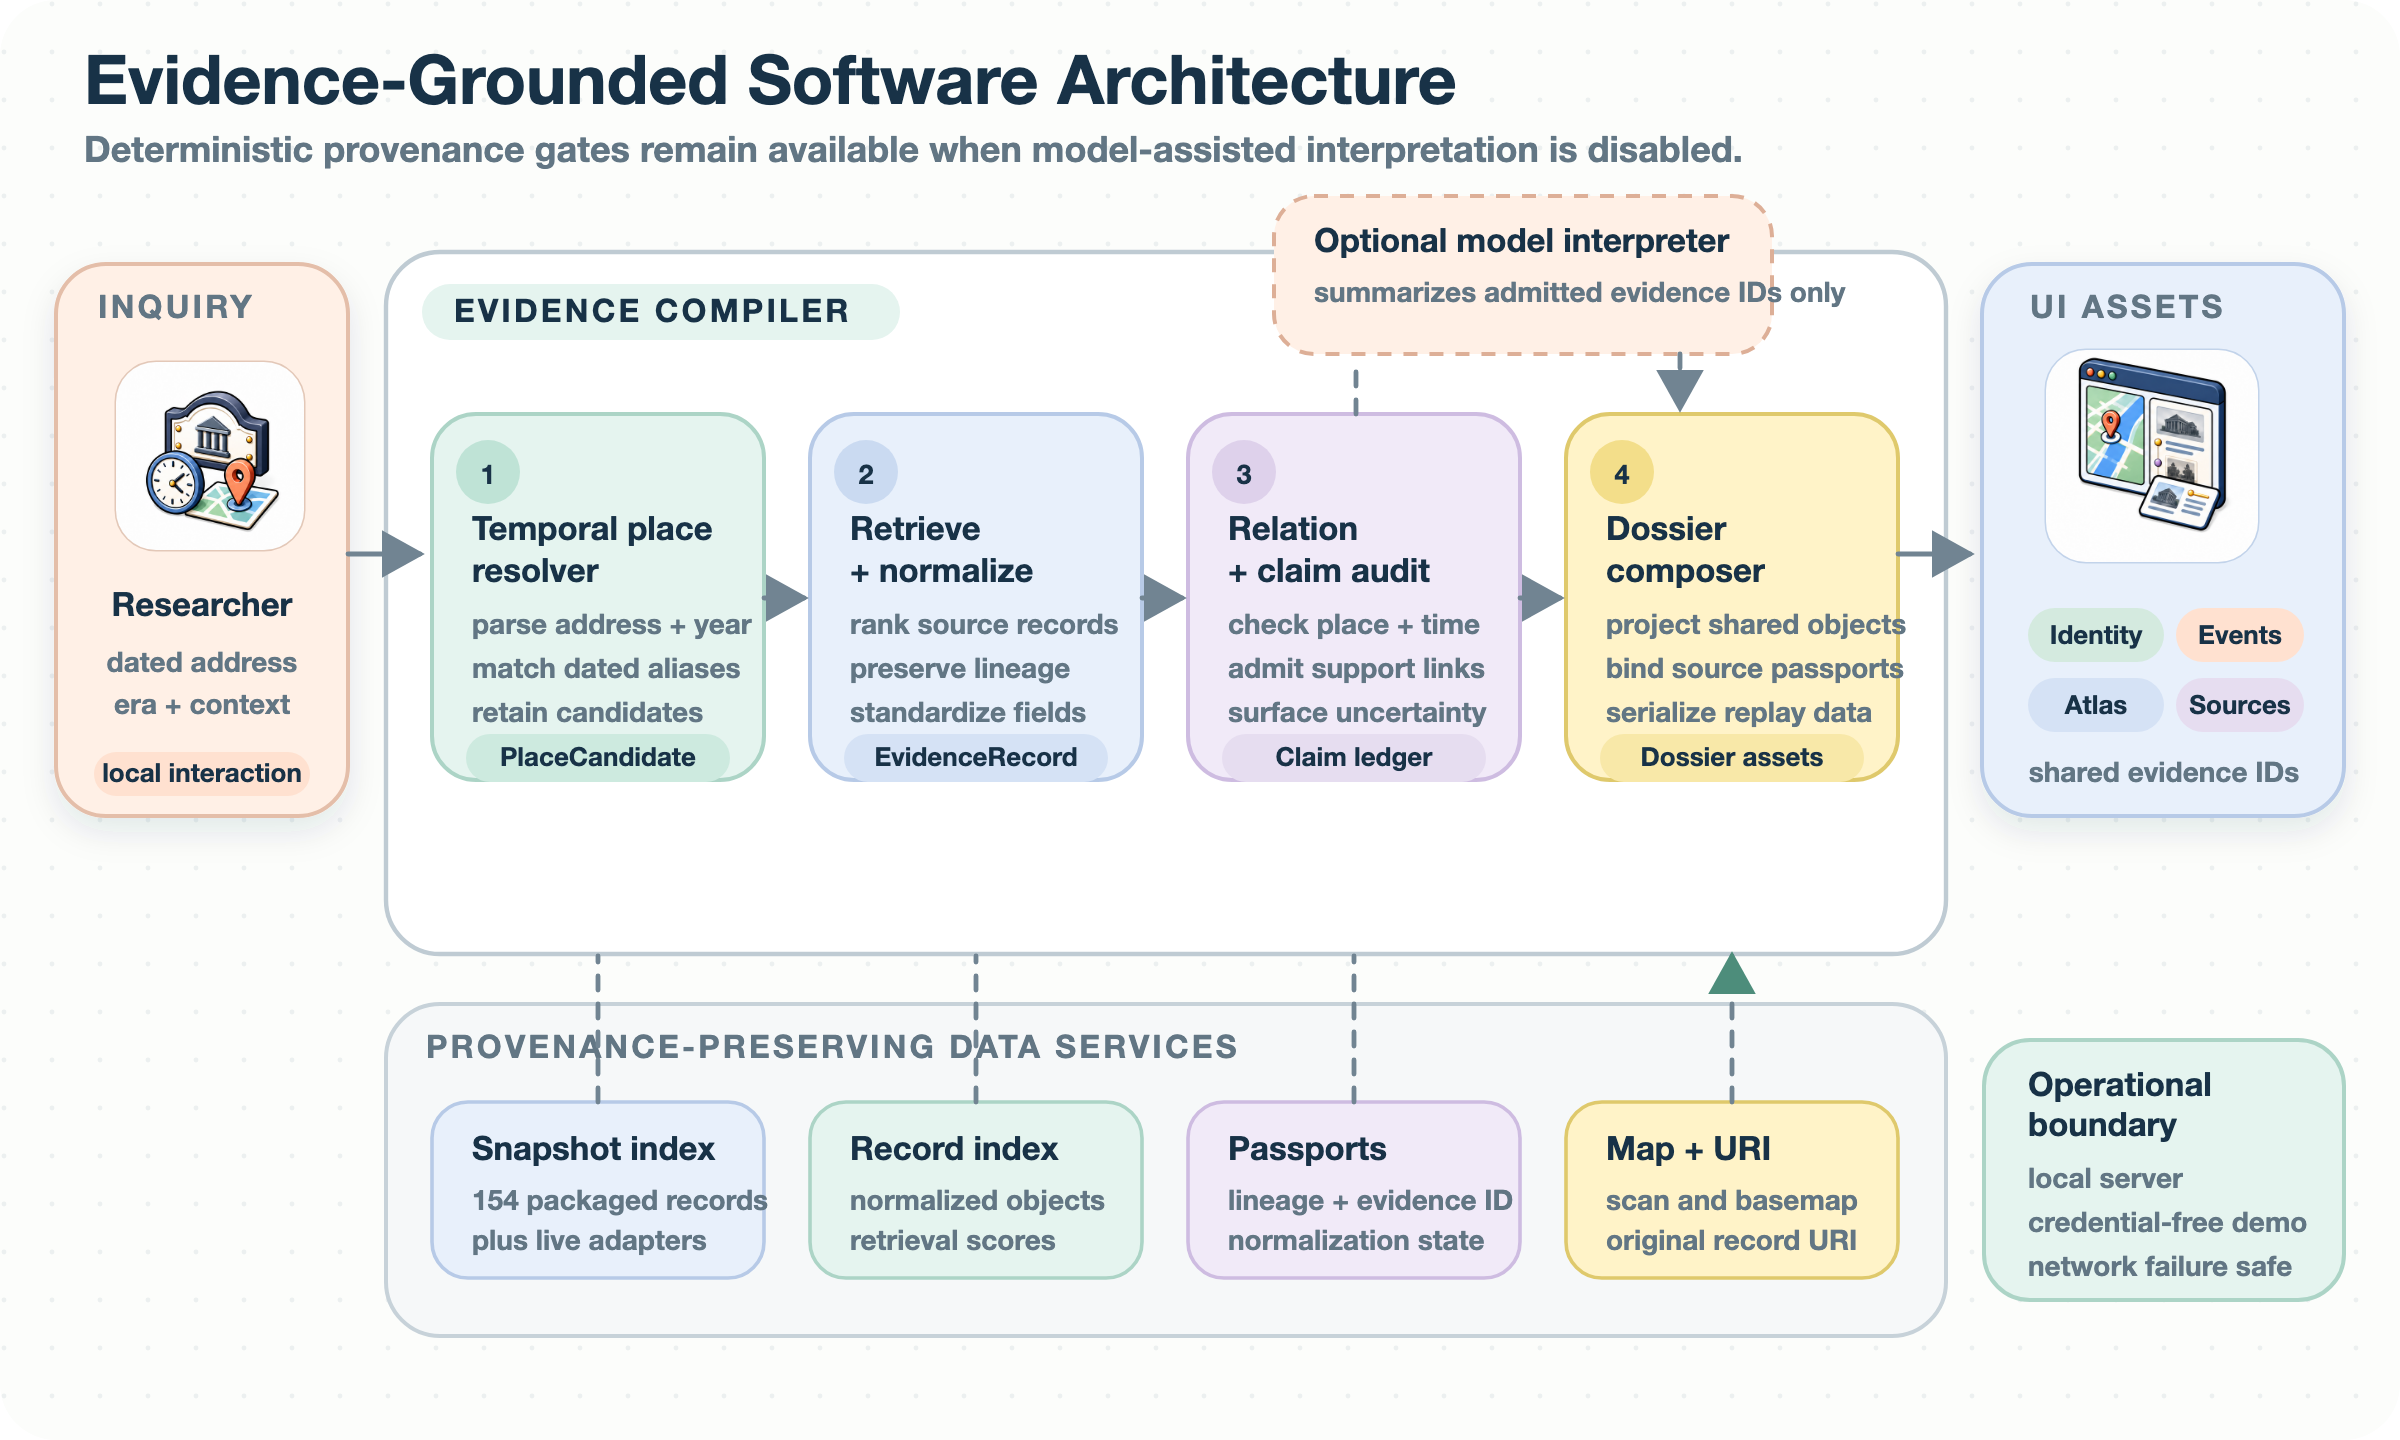
\includegraphics[width=\linewidth]{figures/contextlens_architecture.png}\par\vspace{0.18cm}
\figcap{1}{A deterministic compiler mediates between dated inquiry, provenance-preserving data services, and four interface views. The optional language model receives admitted evidence IDs only.}

\sectiongap
\sectionhead{Source-to-interface data flow}
\centering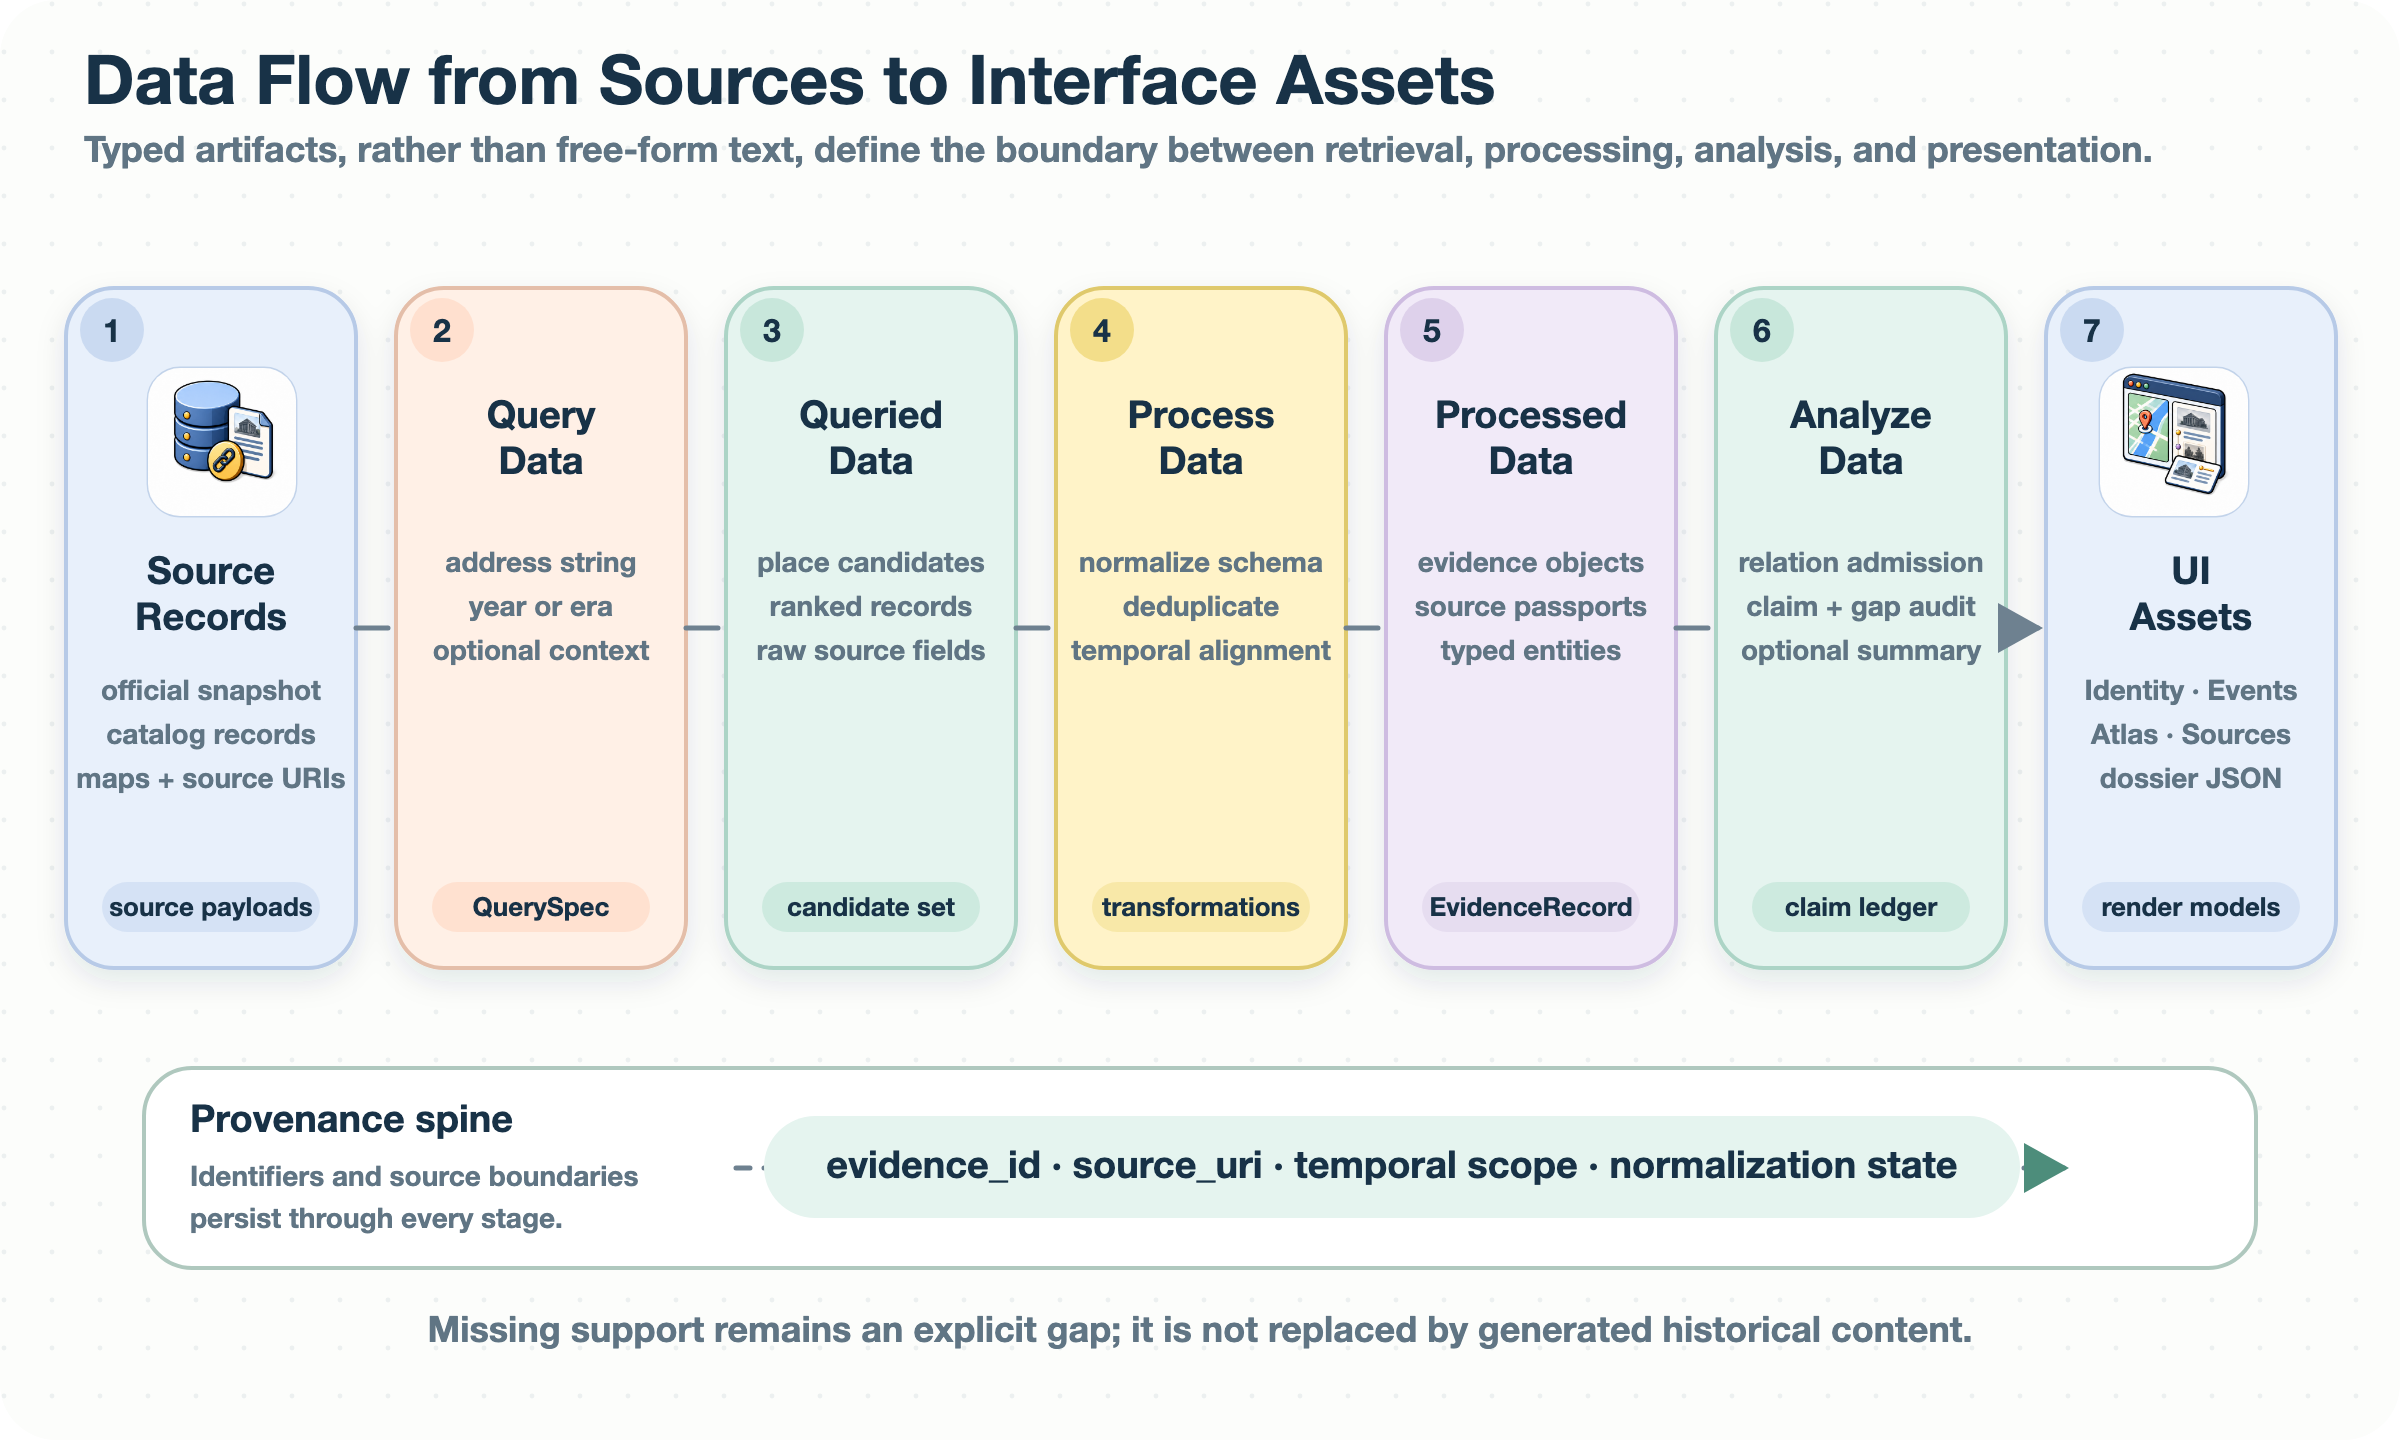
\includegraphics[width=\linewidth]{figures/contextlens_data_flow.png}\par\vspace{0.18cm}
\figcap{2}{Typed artifacts carry evidence\_id, source\_uri, temporal scope, and normalization state from source records to the rendered dossier.}

\sectiongap
\sectionhead{Data and provenance}
\justifying
The packaged snapshot contains \textbf{154 verified records} from Shanghai Library data families covering road and place names, historical events, buildings, people, and organizations. Dated names establish identity; events support direct claims; buildings, people, and organizations add bounded context.\par\vspace{0.25cm}
\lead{Preservation rule.}{Normalization never erases the provider boundary. Every admitted record retains its evidence ID, dataset, time span, normalization status, and official URI.}\par\vspace{0.25cm}
\lead{Model boundary.}{A model may summarize admitted records, but disabling it---or losing network access---does not change the deterministic dossier.}\par\vspace{0.25cm}
\lead{Audit trail.}{The dossier JSON and the four interface views project the same typed evidence objects, allowing a reviewer to trace a displayed statement without reconstructing hidden intermediate steps.}

\sectiongap
\sectionhead{Design principles and scope}
\principle{01}{Resolve before retrieval}{Historical place identity is a prerequisite for evidence collection, not an afterthought.}{PosterBlue}
\principle{02}{Expose uncertainty}{Ambiguous candidates and missing support remain visible to the investigator.}{PosterOrange}
\principle{03}{Avoid false precision}{The 1943 scan supports orientation, not exact house-number alignment.}{PosterRed}
\principle{04}{Bound evaluation claims}{The paper reports implementation tests; it does not claim retrieval accuracy or a completed user study.}{PosterGreen}

\colorbox{PosterPaleTwo}{\parbox{0.96\linewidth}{\vspace{0.2cm}\lead{Why this matters for digital history.}{Historical investigation moves repeatedly between names, dates, maps, and source records. ContextLens makes those transitions explicit in one artifact. It is an investigation interface, not a general geocoder or unconstrained question-answering system.}\vspace{0.2cm}}}
\end{minipage}
\end{column}

\begin{column}{0.018\textwidth}\centering\color{PosterLine}\rule{0.05cm}{98.4cm}\end{column}

% -----------------------------------------------------------------------------
\begin{column}{0.318\textwidth}
\bodyfont\justifying
\begin{minipage}[t][98.4cm][s]{\linewidth}

\sectionhead{Demonstration}
{\fontsize{29}{33}\selectfont\bfseries\color{PosterNavy}436 Avenue Joffre, 1934}\par\vspace{0.25cm}
The resolver associates Avenue Joffre with the present-day Huaihai Middle Road area. It reconstructs six dated road names and connects the 1934 founding of Kangjian Bookstore to No. 436. The event claim remains bounded by its supporting record and temporal scope.

\vspace{0.25cm}
\lead{Investigation task.}{The attendee can inspect the selected identity, compare admitted and contextual records, and reopen the official source behind each direct claim.}

\vspace{0.35cm}
\colorbox{PosterPale}{\parbox{0.96\linewidth}{\centering\bfseries\color{PosterBlue} Identity first $\rightarrow$ evidence gates $\rightarrow$ coordinated dossier}}

\sectiongap
\sectionhead{Query-to-dossier workflow}
\centering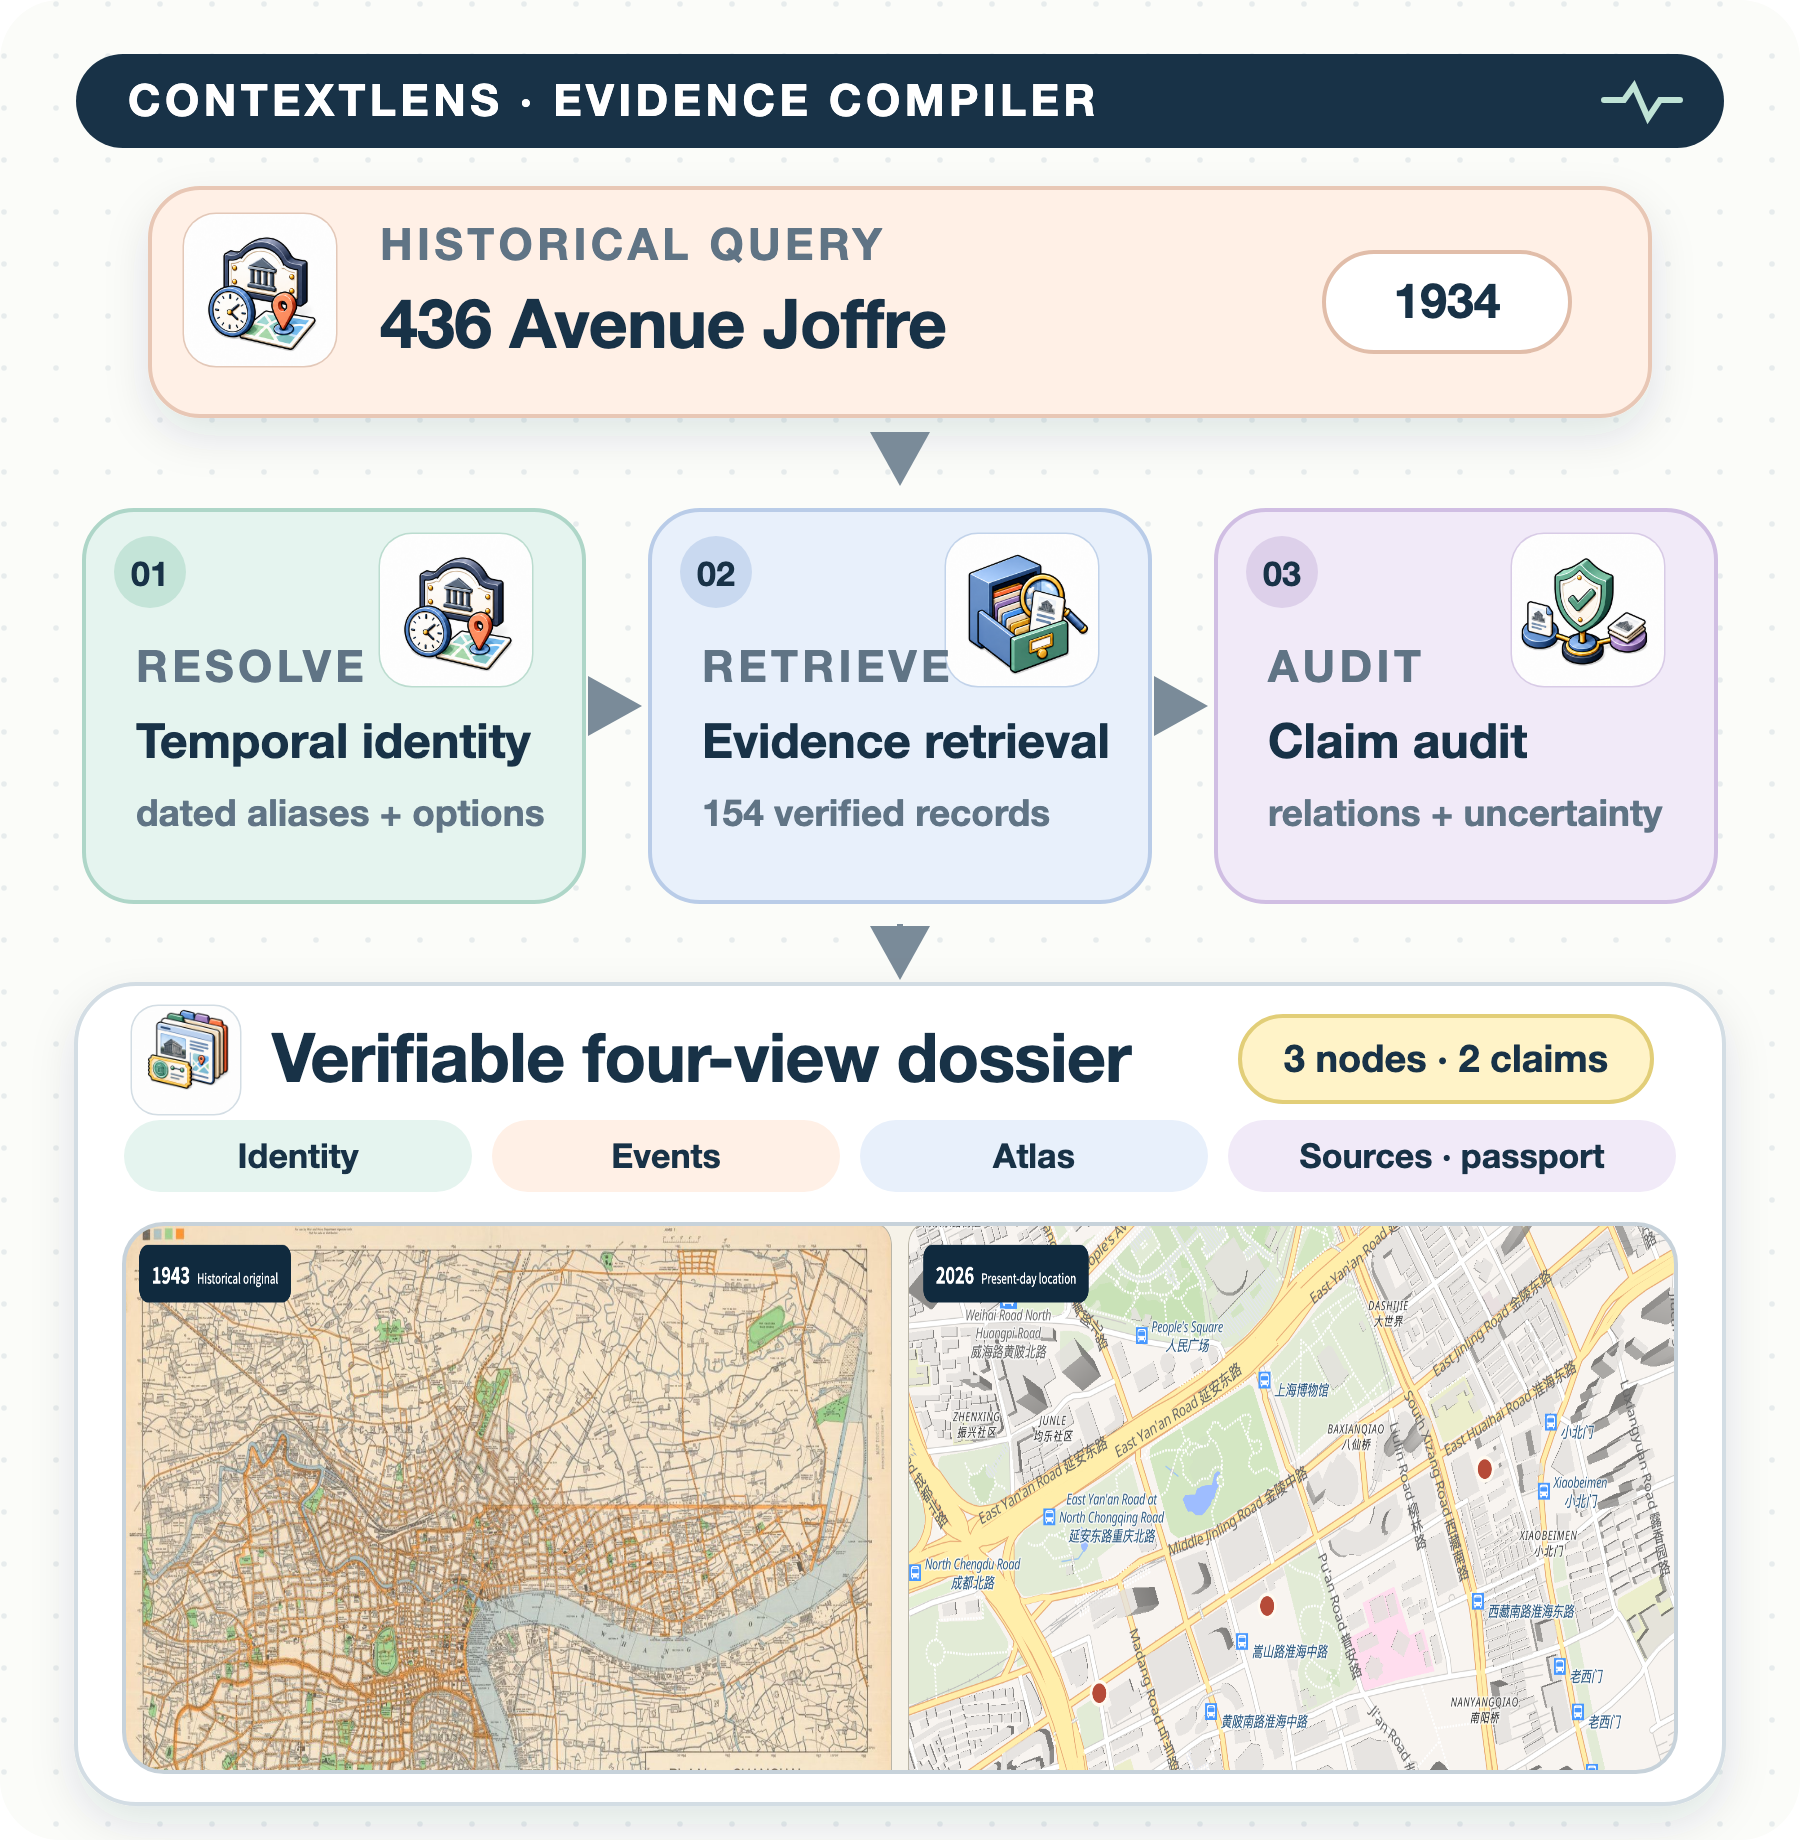
\includegraphics[height=31.5cm,width=\linewidth,keepaspectratio]{figures/contextlens_teaser.png}\par\vspace{0.18cm}
\figcap{3}{A dated query is resolved before retrieval. Relation and claim gates determine which records may support the Identity, Events, Atlas, and Sources views.}

\sectiongap
\sectionhead{Main-case output}
\begin{beamercolorbox}[wd=\linewidth,sep=0.35cm]{metrics}
  \begin{minipage}[t]{0.19\linewidth}\centering{\fontsize{32}{35}\selectfont\bfseries\color{PosterBlue}6}\par{\fontsize{16}{19}\selectfont dated road\\names}\end{minipage}\hfill
  \begin{minipage}[t]{0.19\linewidth}\centering{\fontsize{32}{35}\selectfont\bfseries\color{PosterCyan}3}\par{\fontsize{16}{19}\selectfont spatiotemporal\\nodes}\end{minipage}\hfill
  \begin{minipage}[t]{0.19\linewidth}\centering{\fontsize{32}{35}\selectfont\bfseries\color{PosterGreen}2}\par{\fontsize{16}{19}\selectfont direct\\claims}\end{minipage}\hfill
  \begin{minipage}[t]{0.19\linewidth}\centering{\fontsize{32}{35}\selectfont\bfseries\color{PosterOrange}4}\par{\fontsize{16}{19}\selectfont evidence\\cards}\end{minipage}\hfill
  \begin{minipage}[t]{0.19\linewidth}\centering{\fontsize{32}{35}\selectfont\bfseries\color{PosterRed}3}\par{\fontsize{16}{19}\selectfont supporting\\records}\end{minipage}
\end{beamercolorbox}
\vspace{0.28cm}
Counts describe the returned dossier for one address; they are not confused with the 154-record snapshot. Each direct claim is connected to an openable evidence card, while contextual records remain distinguishable from supporting evidence.

\sectiongap
\sectionhead{Temporal lineage}
The interface retains each dated label rather than collapsing history into one modern road name.\par\vspace{0.35cm}
\begin{tikzpicture}[x=1cm,y=1cm]
  \draw[PosterLine,line width=2.2pt] (0.5,0) -- (0.5,-16.2);
  \foreach \y/\period/\name/\col in {
    0/{1901--1906}/{Xijiang Road}/PosterBlue,
    -3/{1906--1915}/{Baochang Road}/PosterBlue,
    -6/{1915--1943}/{Avenue Joffre}/PosterOrange,
    -9/{1943--1945}/{Taishan Road}/PosterBlue,
    -12/{1945--1950}/{Linsen Middle Road}/PosterBlue,
    -15/{1950--present}/{Huaihai Middle Road}/PosterBlue}
  {
    \fill[\col] (0.5,\y) circle (0.25);
    \node[anchor=west,text=\col,font=\fontsize{20}{24}\selectfont\bfseries] at (1.4,\y) {\period};
    \node[anchor=west,text=PosterInk,font=\fontsize{20}{24}\selectfont] at (8.2,\y) {\name};
  }
  \node[anchor=west,text=PosterOrange,font=\fontsize{20}{24}\selectfont\itshape] at (8.2,-7.0) {query year: 1934};
\end{tikzpicture}

\sectiongap
\sectionhead{Atlas and coordinated views}
\centering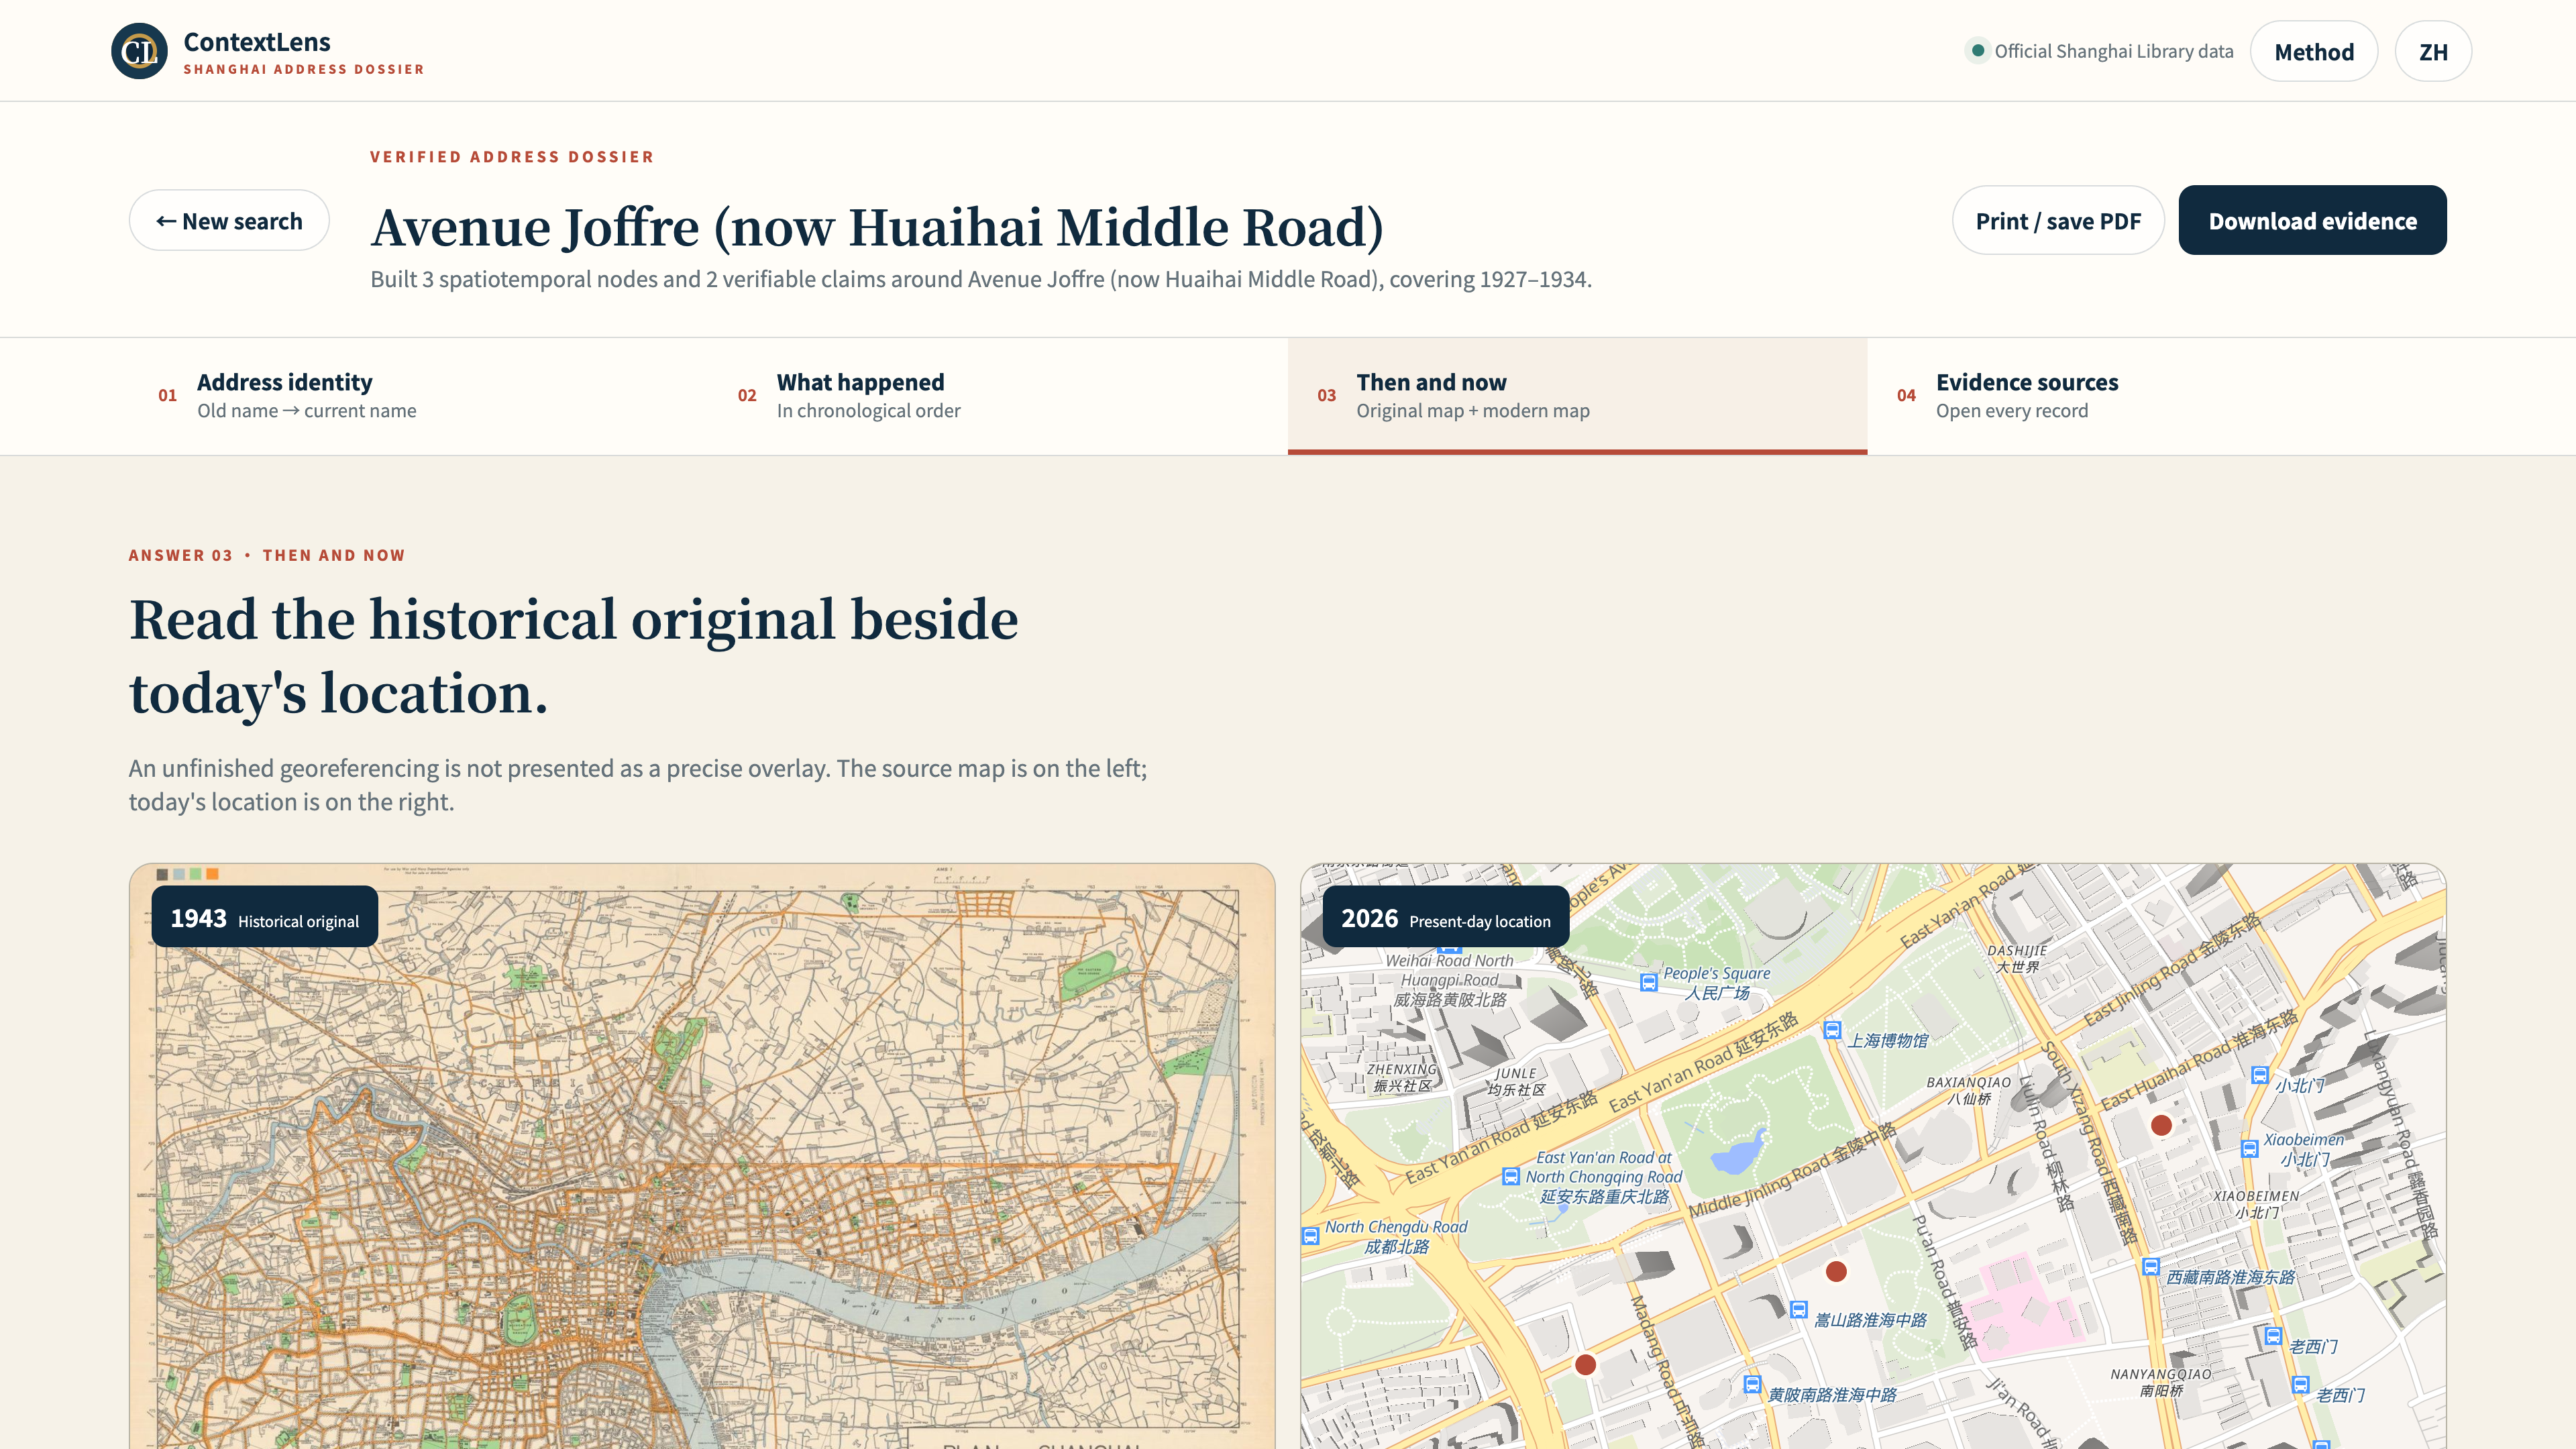
\includegraphics[width=\linewidth]{figures/contextlens_atlas.png}\par\vspace{0.18cm}
\figcap{4}{The Atlas places a 1943 scan beside a present-day map. The archival scan is orientation evidence and does not imply exact house-number alignment.}
\vspace{0.3cm}\justifying
\lead{Coordinated inspection.}{Identity, Events, Atlas, and Sources reference the same spatiotemporal nodes and evidence identifiers. Moving between views changes presentation, not the evidential objects underneath.}\par\vspace{0.25cm}
\lead{Human judgment remains central.}{The interface exposes candidate identity, temporal scope, and source lineage so an investigator can accept, reject, or revisit the compilation.}
\end{minipage}
\end{column}

\begin{column}{0.018\textwidth}\centering\color{PosterLine}\rule{0.05cm}{98.4cm}\end{column}

% -----------------------------------------------------------------------------
\begin{column}{0.318\textwidth}
\bodyfont\justifying
\begin{minipage}[t][98.4cm][s]{\linewidth}

\sectionhead{Claim-level provenance}
{\fontsize{25}{29}\selectfont\bfseries\color{PosterNavy}A Source Passport keeps provenance as interface data}\par\vspace{0.25cm}
A reported claim and its evidence card share one identifier. The user can inspect how the source entered the dossier, verify its temporal limits, and follow the original URI [4--6]. This shifts citation from a decorative endpoint to an interactive part of reasoning.

\sectiongap
\sectionhead{Sources interaction}
\centering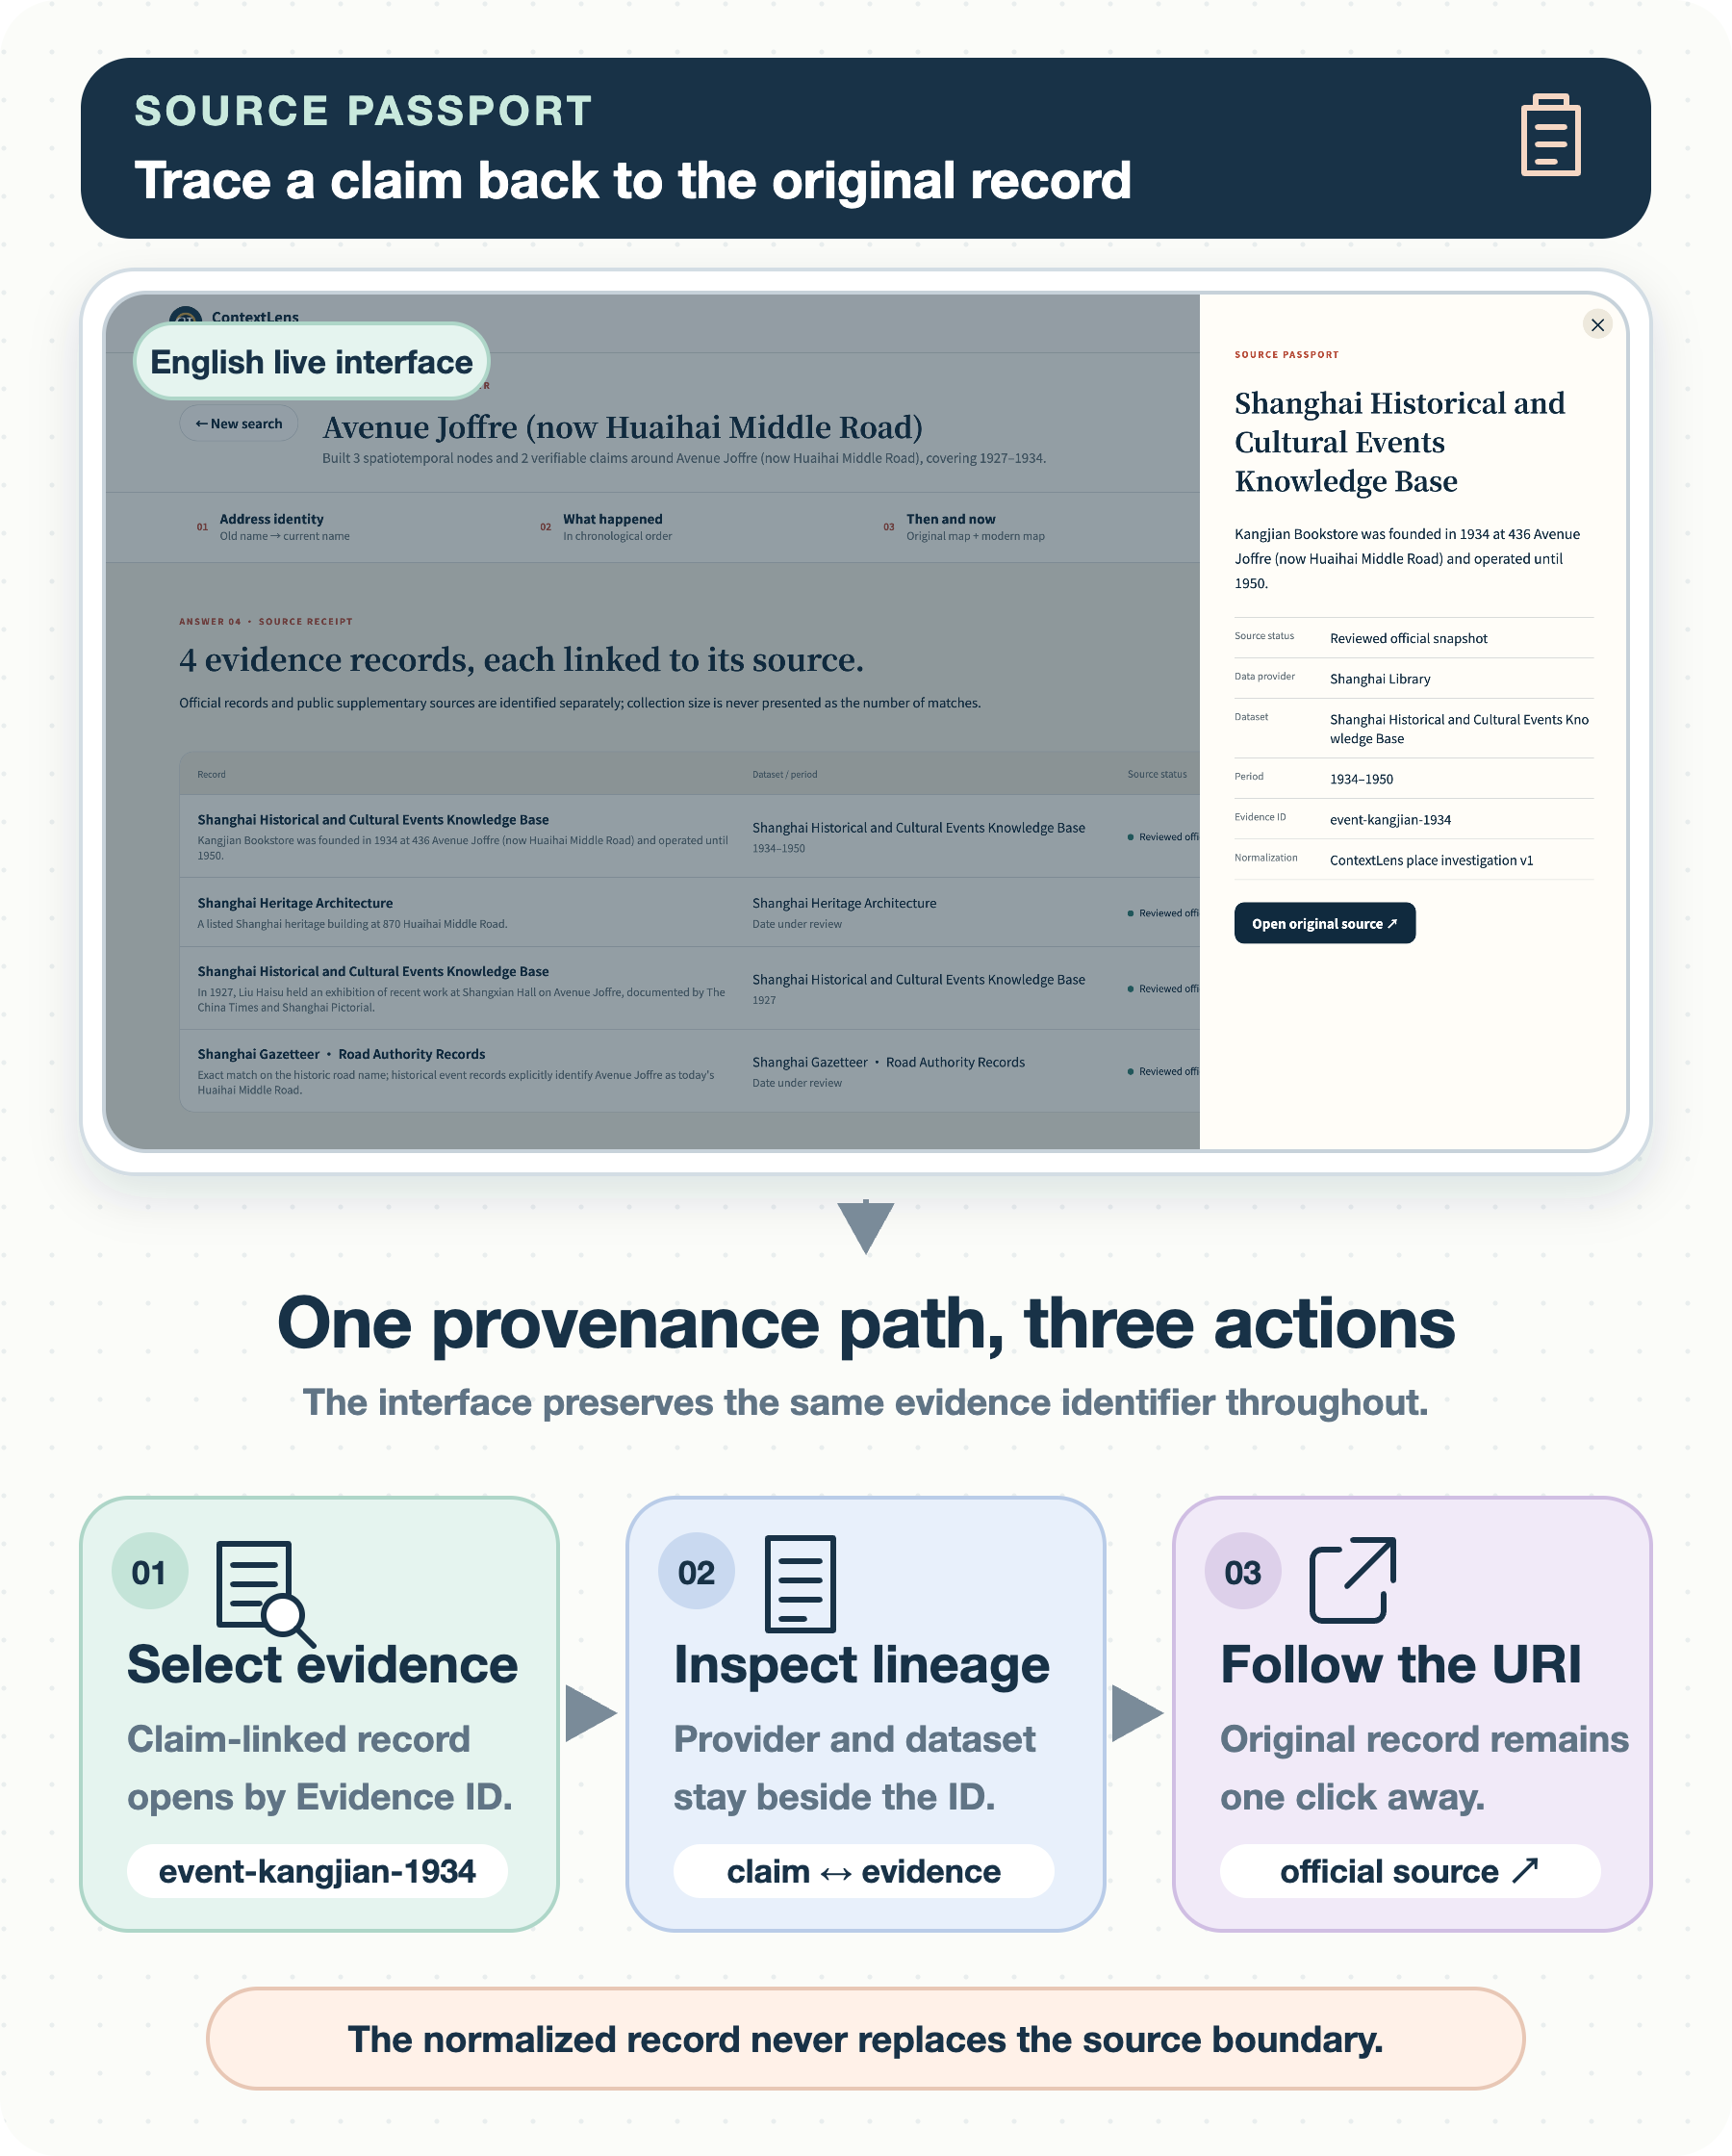
\includegraphics[height=35.5cm,width=\linewidth,keepaspectratio]{figures/contextlens_sources_figure.png}\par\vspace{0.18cm}
\figcap{5}{Selecting a claim-linked record opens its Source Passport. The same evidence ID remains visible while the user inspects lineage and follows the official source URI.}

\sectiongap
\sectionhead{What the Source Passport records}
\lead{Evidence ID.}{A stable identifier links the direct claim, evidence card, and provenance panel; the main case includes \texttt{event-kangjian-1934}.}\par\vspace{0.27cm}
\lead{Provider and dataset.}{The source boundary remains explicit: a Shanghai Library event record is not presented as a system-generated fact.}\par\vspace{0.27cm}
\lead{Temporal scope.}{Period metadata limits when a record can support a relation; incompatible dates cannot silently become direct evidence.}\par\vspace{0.27cm}
\lead{Normalization and URI.}{Transformation state is exposed, and the user can reopen the official record rather than relying on the interface summary alone.}\par\vspace{0.28cm}
{\centering\itshape\color{PosterRed}Identifier gating can reject unsupported citations, but it cannot by itself establish the historical adequacy of a source record.\par}

\vspace{0.28cm}
\lead{Cross-view consistency.}{Identity, Events, Atlas, Sources, and the exported dossier reuse the admitted evidence set; changing views does not create a separate or less constrained account of the case.}

\sectiongap
\sectionhead{Reproducibility}
\begin{beamercolorbox}[wd=\linewidth,sep=0.35cm]{repro}
  \begin{minipage}[t]{0.31\linewidth}\centering{\fontsize{30}{33}\selectfont\bfseries\color{PosterBlue}154}\par{\fontsize{16}{19}\selectfont verified snapshot\\records}\end{minipage}\hfill
  \begin{minipage}[t]{0.31\linewidth}\centering{\fontsize{30}{33}\selectfont\bfseries\color{PosterGreen}29/29}\par{\fontsize{16}{19}\selectfont Python test\\functions pass}\end{minipage}\hfill
  \begin{minipage}[t]{0.31\linewidth}\centering{\fontsize{30}{33}\selectfont\bfseries\color{PosterOrange}PASS}\par{\fontsize{16}{19}\selectfont TypeScript +\\frontend build}\end{minipage}
\end{beamercolorbox}
\vspace{0.28cm}
The reviewed product requires no Shanghai Library API key, model key, or Node.js runtime. Resolution, claim gating, provenance, privacy behavior, ambiguity, unresolved queries, and network failure are covered by implementation tests.

\sectiongap
\sectionhead{Failure-aware behavior}
\principle{A}{Ambiguous input}{``Nanjing Road department store'' retains East and West Nanjing Road candidates for inspection.}{PosterOrange}
\principle{B}{Unknown address}{``9999 Mars Road'' remains unresolved and requests more evidence instead of inventing a match.}{PosterRed}
\principle{C}{Network or model failure}{The verified local dossier remains available; optional summarization cannot introduce a new evidence ID.}{PosterGreen}

\sectiongap
\sectionhead{Limitations and evaluation agenda}
The current snapshot is Shanghai-specific and small relative to the underlying collections. Dated name rules require maintenance, some coordinates remain coarse, and the prototype has not yet completed a historian or public-user study.\par\vspace{0.28cm}
\lead{Next evaluation.}{Resolution benchmarks should measure candidate ranking, temporal consistency, and abstention. Expert correction workflows should capture revised name periods, coordinates, and evidential judgments.}

\sectiongap
\sectionhead{AAAI demonstration relevance}
The live demonstration makes evidence grounding observable: attendees can issue a dated place query, inspect a resolved lineage, open claim-linked records, compare historical and current maps, and deliberately trigger ambiguous or unresolved cases. The system's behavior is therefore examinable at each decision boundary, including failure.
\end{minipage}
\end{column}
\end{columns}
\end{frame}
\end{document}
